% This file was created with tikzplotlib v0.10.1.
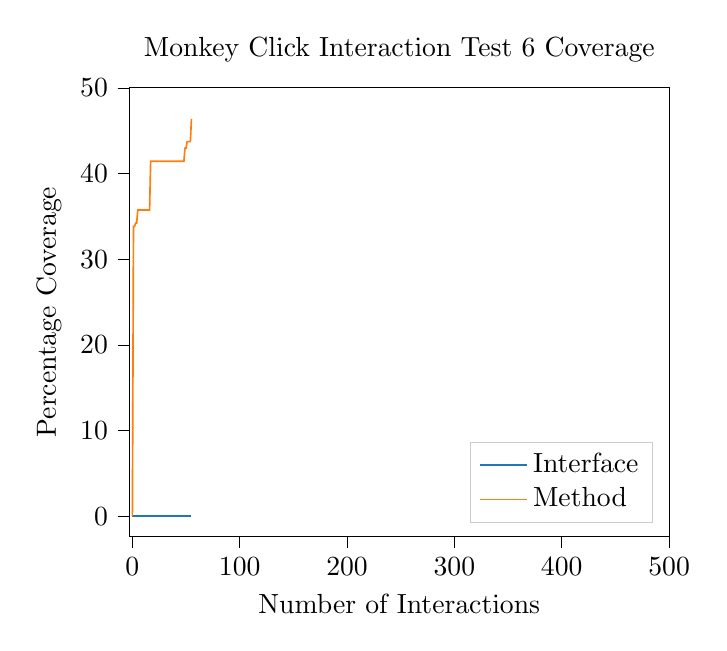
\begin{tikzpicture}

\definecolor{darkgray176}{RGB}{176,176,176}
\definecolor{darkorange25512714}{RGB}{255,127,14}
\definecolor{lightgray204}{RGB}{204,204,204}
\definecolor{steelblue31119180}{RGB}{31,119,180}

\begin{axis}[
legend cell align={left},
legend style={
  fill opacity=0.8,
  draw opacity=1,
  text opacity=1,
  at={(0.97,0.03)},
  anchor=south east,
  draw=lightgray204
},
tick align=outside,
tick pos=left,
title={Monkey Click Interaction Test 6 Coverage},
x grid style={darkgray176},
xlabel={Number of Interactions},
xmin=-2.75, xmax=500,
xtick style={color=black},
y grid style={darkgray176},
ylabel={Percentage Coverage},
ymin=-2.3195, ymax=50,
ytick style={color=black}
]
\addplot [semithick, steelblue31119180]
table {%
0 0
1 0
2 0
3 0
4 0
5 0
6 0
7 0
8 0
9 0
10 0
11 0
12 0
13 0
14 0
15 0
16 0
17 0
18 0
19 0
20 0
21 0
22 0
23 0
24 0
25 0
26 0
27 0
28 0
29 0
30 0
31 0
32 0
33 0
34 0
35 0
36 0
37 0
38 0
39 0
40 0
41 0
42 0
43 0
44 0
45 0
46 0
47 0
48 0
49 0
50 0
51 0
52 0
53 0
54 0
55 0
};
\addlegendentry{Interface}
\addplot [semithick, darkorange25512714]
table {%
0 0
1 33.84
2 33.84
3 34.22
4 34.22
5 35.74
6 35.74
7 35.74
8 35.74
9 35.74
10 35.74
11 35.74
12 35.74
13 35.74
14 35.74
15 35.74
16 35.74
17 41.44
18 41.44
19 41.44
20 41.44
21 41.44
22 41.44
23 41.44
24 41.44
25 41.44
26 41.44
27 41.44
28 41.44
29 41.44
30 41.44
31 41.44
32 41.44
33 41.44
34 41.44
35 41.44
36 41.44
37 41.44
38 41.44
39 41.44
40 41.44
41 41.44
42 41.44
43 41.44
44 41.44
45 41.44
46 41.44
47 41.44
48 41.44
49 42.97
50 42.97
51 43.73
52 43.73
53 43.73
54 43.73
55 46.39
};
\addlegendentry{Method}
\end{axis}

\end{tikzpicture}
